\documentclass[10pt,a4paper]{article}
\usepackage[T1]{fontenc}
\usepackage{charter}
\usepackage{inconsolata}
\usepackage{geometry}
\usepackage{graphicx}
\usepackage{caption}
\usepackage{subcaption}
\usepackage{rotating}
\usepackage{gensymb}
\usepackage{tikz}
\usetikzlibrary{arrows,positioning,shapes}

\usetikzlibrary{external}
\tikzexternalize[
  mode=list and make,
  prefix=figures/]

\usepackage{booktabs}
\geometry{left=0.5in,right=0.5in,top=0.5in,bottom=1in,a4paper}
\setlength{\parskip}{2ex plus 0.5ex minus 0.5ex}
\setlength{\parindent}{0pt}
\def\gap{\hspace{2cm}}
\usepackage[charter]{mathdesign}
\usepackage{amsmath}
\usepackage[draft]{hyperref}
\title{OS grid reference and height from a phone's GPS\\by fast approximations}
\author{Richard P. Curnow\\Somewhere in ST 3663}

\tikzset{
    %Define standard arrow tip
    >=stealth',
    %Define style for boxes
    box/.style={
           rectangle,
           rounded corners,
           draw=black, very thick,
           text width=9em,
           minimum height=2em,
           text centered},
    boxzag/.style={
           draw=black, very thick,
           starburst,
           text width=6.5em,
           minimum height=2em,
           text centered},
    annot/.style={
           text width=7em,
           text centered},
    % Define arrow style
    arr/.style={
           ->,
           very thick,
           shorten <=2pt,
           shorten >=2pt,},
    redarr/.style={
           ->,
           very thick,
           draw=red,
           shorten <=2pt,
           shorten >=2pt,},
    bluearr/.style={
           ->,
           very thick,
           draw=blue,
           shorten <=2pt,
           shorten >=2pt,},
    purparr/.style={
           ->,
           very thick,
           draw=blue!50!red,
           shorten <=2pt,
           shorten >=2pt,}
}

\begin{document}
\maketitle
\tableofcontents
\clearpage

\section {Background and aims}
Whilst writing a mapping application to run on an Android phone, the author
wanted two features:
\begin{enumerate}
\item To display height above sea level, having noticed that the `height'
provided by the GPS was somewhat higher than the figure shown on maps
\item To display the OS grid reference of a point on the map
\end{enumerate}

The basic method described in the Ordnance Survey documentation (ref [1]) for
these conversions involve a significant amount of calculation --- see for
example figure \ref{fig:derivation_helmert} and section \ref{sec:os_models} of
this note.  Even then, the positional accuracy is quoted as no better than 5
metres\footnote{due to the use of the Helmert transformation step}.  To get
greater accuracy, the OS provide the reference models OSTN02 (for position) and
OSGM02 (for height).  These are effectively a pair of look-up tables modelling
the displacement of a ``rubber sheet'' at 1km intervals.  The text file
containing the models is 37 megabytes in size.  The lookup-table method still
requires use of the substantial calculation\footnote{It is the transverse
Mercator projection from WGS84 latitude \& longitude to an eastings, northings
coordinate pair} in annex C.1 of \cite{gcs}.  Consequently, neither of the
approaches provided by the OS was considered suitable to embed into an Android
application --- in view of both the work in the annex C.1 calculation, and then
the trade-off of accuracy versus storage and RAM needed for the OSTN02/OSGM02
database.

This note describes the results of looking for an alternative method.  The
target accuracy in grid position was to achieve no worse than 10 metres in the
grid reference, but ideally to reach an accuracy that would be negligible
compared to the accuracy of the position provided by the phone's GPS, if the
resulting computation was still cheap enough to do.  The target for height was
arbitrary in view of the poor accuracy of the height given by low-end GPS
receivers -- a `best endeavours' approach.

The two approximations being sought are the red arrows shown in figure
\ref{fig:aims}.  The GPS device provides WGS84 (lat,long,height) coordinates.
Within the Android application being developed, the (lat,long) are converted
early to Web Mercator coordinates.  This representation is used throughout the
map drawing part of the program.

The first desired approximation is a formula to get the height above mean sea
level, relative to the UK datum at Newlyn, from the WGS84 coordinates, for text
display.

The second desired approximation is to get from Web Mercator coordinates to an
OS grid reference (Eastings, Northings).  Web Mercator was the chosen domain
for the approximation because it is desired to show the grid reference of any
location as the map is panned, without converting back to lat,long.

% ----------------------------------------------------------------------------
\begin{figure}[htbp]
  \hrulefill

  \centering
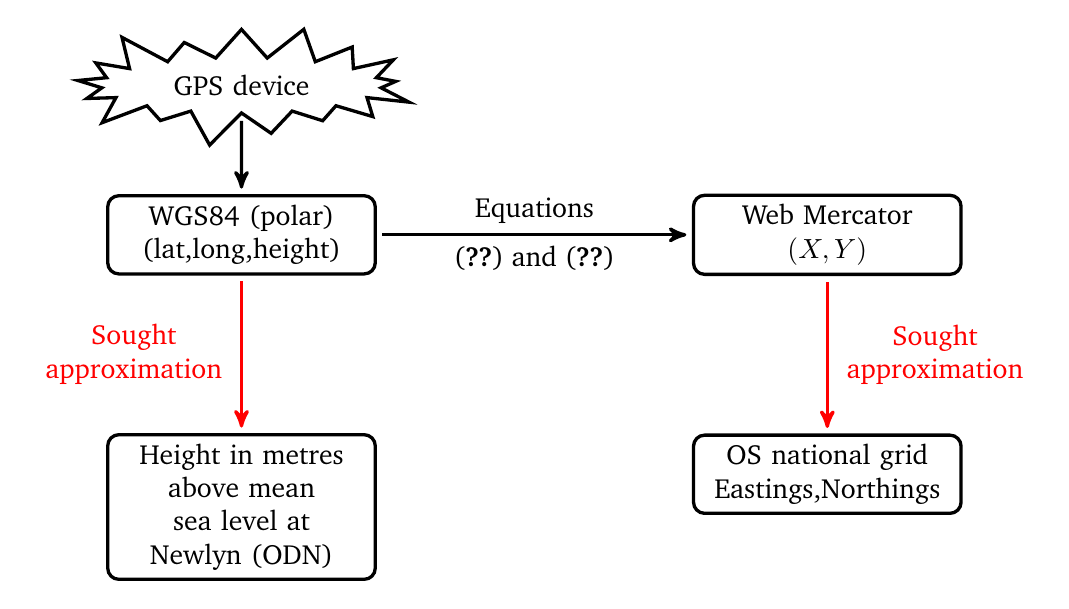
\begin{tikzpicture}
  \begin{scope}
  \node[box] (wgs84-polar) {WGS84 (polar) \linebreak (lat,long,height)};
  \node[box, right=4cm of wgs84-polar] (wm) {Web Mercator \linebreak $(X,Y)$};
  \path [arr,->] (wgs84-polar)
    edge
      node[above]{Equations}
      node[below]{\eqref{eqn:wmx} and \eqref{eqn:wmy}}
        (wm);
  \node[boxzag, above=of wgs84-polar] ((gps) {GPS device}
    edge[arr,->] (wgs84-polar.north);
  \node[box, below=2cm of wgs84-polar] (odn) {Height in metres above mean sea level at Newlyn (ODN)}
    edge[redarr,<-] node[annot,left,red]{Sought\\approximation}
      (wgs84-polar.south);
  \node[box, below=2cm of wm] (en) {OS national grid \linebreak Eastings,Northings}
    edge[redarr,<-] node[annot,right,red]{Sought\\approximation}
      (wm.south);
  \end{scope}
\end{tikzpicture}
\caption{The approximations that the work aims to find}
\label{fig:aims}

  \hrulefill
\end{figure}
% ----------------------------------------------------------------------------

\section {Adjusting WGS84 elevation to give ODN height}
Assume $M_d$ and $L_d$ are the latitude and longitude in \textbf{degrees}
(positive $M_d$ is north, positive $L_d$ is east).  Define $P$, $Q$ as follows:

\begin{align}
P & = \frac{2\left(M_d - 54.5\right)}{9} \\
  Q & = \frac{\left(L_d + 2.0\right)}{4}
\end{align}

The $(P,Q)$ coordinate system is centred on (54.5\degree{}N, 2\degree{}W)
\footnote{on Low Green Fell south of Bowes --- a tranquil- and bleak-looking
spot in the Pennines}
and $P$ and $Q$ run over approximately $[-1,1]$ for the $M_d \in [50,59]$, $L_d
\in [-6,+2]$ ranges spanning most of the UK.\footnote{The reason for forcing
$P$ and $Q$ into the range $[-1,1]$ is to make it easier to see which
higher-order terms have no relevant effect on the result and can be dropped.}

Then if $W$ is the elevation from WGS84 (as read from a GPS device) and $A$ is
the height above mean sea level referenced to Newlyn
\footnote{$A$ for \textbf{actual}, $W$ for \textbf{WGS84}},
the height difference $\Delta H = A-W$ can be approximated using the following
rather simple formula:

\begin{align}
  \Delta H(P,Q) &= -50.1 + 6.1Q - 1.1P - 1.5 PQ
  \label{eqn:odn}
\end{align}

Then, given a $(M_d,L_d,W)$ tuple from a phone's GPS, the ``height above sea
level'' (referenced to ODN) can be estimated as

\begin{equation}
\hat{A} = W + \Delta H(P,Q)
\label{eqn:ahat}
\end{equation}

where $P$ and $Q$ are obtained from $M_d$ and $L_d$ as shown earlier.

The coefficients in equation \eqref{eqn:odn} were arrived at by a least-squares
fit against the OSGM02 model on a grid of points in the lat,long space.  Note
that the value is negative --- the WGS84 ellipsoid, which GPS heights are given
against, is beneath the geoid over the UK so GPS heights are too high.

The error between $\hat{A}$ given by equation \eqref{eqn:ahat} and the OSGM02
model is shown in figure \ref{fig:odn_base} on page \pageref{fig:odn_base}.  The worst
error is about 3 metres at Land's End.  Given that the height accuracy of a
phone's GPS is quoted as being far worse than this, and only an approximate
height above sea level was sought, this approximation was considered
sufficient, especially as equation \eqref{eqn:odn} is so cheap to evaluate.
Table \ref{tbl:contour_key} on page \pageref{tbl:contour_key} shows the
representations of the contours.

% ----------------------------------------------------------------------------
\begin{figure}[t]
  \centering
  \fbox{
    \input picture2
  }
  \caption{Web Mercator zoom-6 tiles with stretched OS grid overlaid}
  \label{fig:grid_os}
\end{figure}
% ----------------------------------------------------------------------------

\section {Conversion between Web Mercator and OS national grid}

\subsection {Web Mercator}
Web Mercator is the system used for indexing the tiles on web-based map servers
such as OpenStreetMap.  Given latitude $M$ and longitude $L$, in
\textbf{radians} with north and east positive, the formulae are 

\begin{align}
  X & = \frac{1}{2}\left(1 + \frac{L}{\pi} \right) \label{eqn:wmx} \\
  Y & = \frac{1}{2}\left(1 - \frac{
       \ln\left(\tan{M} + \sec{M}\right)
     }{\pi} \right) \label{eqn:wmy} \\
    \textbf{alternatively } Y & = \frac{1}{2} \left(
        1 - \frac{1}{\pi} \ln \left(
          \frac{1 + \sin{M}}{\cos{M}}
        \right)
        \right)
\end{align}

These formulae return $X$ and $Y$ as fractional values in the range $[-1,1)$.
The $Y$ formula is only used up to latitudes of approximately 85 degrees, so
$Y$ does not go outside the $[-1,1)$ range.

To find the OSM tile number $(t_x,t_y)$ containing the point at zoom level $z$,
the formulae are

\begin{align}
  t_x &= \lfloor 2^z \cdot X \rfloor \\
  t_y &= \lfloor 2^z \cdot Y \rfloor
\end{align}

Inside an application, it is convenient to represent positions in this
coordinate system, in particular as integers given by scaling $X$ and $Y$ by a
power of 2.  This reduces the calculation of tile numbers and pixel offsets to
fast shift and mask operations.  Map tiles downloaded from OSM and Bing are all
indexed relative to this projection.

% ----------------------------------------------------------------------------
\begin{figure}[t]
  \centering
  \fbox{
    \input picture1
  }
  \caption{OS grid with stretched Web Mercator zoom-6 tiles overlaid}
  \label{fig:grid_wm}
\end{figure}
% ----------------------------------------------------------------------------


\subsection {OS grid reference}
OS grid references can be expressed in all-numeric format, in metres of
``easting'' and ``northing'' relative to a false origin off the Cornish coast.
The letters in the usual representation (e.g. AA 123 456) are associated with
the 100000 digit in the all-numeric form --- there is a simple conversion
between the two.  The false origin's location is 100km north and 400km west of
the OSGB36 true origin at 49N, 2W, in the English Channel.  The purpose of the
false origin is to make all coordinates be positive.

The relationship between grid references and Web Mercator is shown in figures
\ref{fig:grid_os} and \ref{fig:grid_wm}.  The black grid is the OS grid.  The
black axis labels are the all-numeric eastings and northings. The letters in
the boxes are the conventional 100km-by-100km grid squares.  The red grid and
labels in figure \ref{fig:grid_os} are Web Mercator, and the green squares are
the 12 tiles at zoom level 6 that cover the UK.  These figures give some idea
of the transformation that has to be approximated --- and the degree of
distortion inherent in the Web Mercator projection.  The small blue circle
shows the position of the $(\alpha,\beta)$ origin used in the following
section.  The blue rectangle shows the region where $\alpha \in [-1,1]$, $\beta
\in [-1,1]$, and over-bounds the area over which the OSTN02 model is defined.

Figure \ref{fig:grid_wm} also shows the relationship between all-numeric and
mixed grid references.  For example, the mixed grid reference ST1234554321 is
equivalent to the all-numeric eastings, northings 312345, 154321.


\subsection {The conversion formula}
Given a point $(X,Y)$ in Web Mercator space, first define $\alpha$ and $\beta$
as scaled X and Y values relative to a point approximately in the middle of a
rectangular region containing the UK.  The point is the centre of the OS grid,
NU0000050000\footnote{about 1 mile south of Berwick-upon-Tweed} mapped back
into Web Mercator space.  $\alpha$ and $\beta$ are calculated as follows:

\begin{align}
  \alpha &= 61 (X-0.494440093) \\
  \beta  &= 36 (Y-0.312663855)
\end{align}

These offsets and scalings ensure that $\alpha$ and $\beta$ are both in the
range $[-1,1]$ over the region including the UK mainland, Orkneys, Shetlands,
Hebrides and Scilly Isles.  This means that any power term $\alpha^m \beta^n$
is also in the range $[-1,1]$, meaning all coeffiencients are easily comparable
in terms of their effect on the values obtained at the edge of the region.  It
is also useful for applying the methods in section \ref{sec:reduction}.  See
section \ref{sec:ab_orig} for a further discussion of the $\alpha,\beta$ origin
and scale factors.

If either $\alpha$ or $\beta$ lies outside the range $[-1,1]$, the location
definitely falls outside the region covered by the OS grid.  In this case, the
conversion can be abandoned with an error.

Then the all-numeric eastings $E$ and northings $N$ can be approximated by
equations \eqref{eqn:east1} and \eqref{eqn:north1} below:

\begin{align}
E_0 &= 400000.70 -17.07\beta -1.74\beta^2\nonumber \\
E_1 &= 370523.38 +53326.92\beta +2025.68\beta^2 -241.27\beta^3 -41.77\beta^4\nonumber \\
E_2 &= 3.28 -19.00\beta +14.84\beta^2 +10.39\beta^3\nonumber \\
E_3 &= -237.68 +77.84\beta +41.21\beta^2 +6.74\beta^3\nonumber \\
E &= E_0 +E_1\alpha +E_2\alpha^2 +E_3\alpha^3
  \label{eqn:east1}
\\[2ex]
N_0 &= 649999.95 -626491.07\beta -44898.33\beta^2 -1105.25\beta^3 +107.47\beta^4 +13.95\beta^5\nonumber \\
N_1 &= -11.56 +4.69\beta^2 -4.53\beta^3\nonumber \\
N_2 &= 15768.99 +1212.74\beta -212.06\beta^2 -53.24\beta^3 -3.43\beta^4\nonumber \\
N_3 &= -3.62 +3.73\beta +11.09\beta^2 -1.28\beta^3\nonumber \\
N_4 &= 12.45 +7.93\beta +2.35\beta^2 +3.65\beta^3 -4.08\beta^4\nonumber \\
N_5 &= -4.81\beta^4\nonumber \\
N &= N_0 +N_1\alpha +N_2\alpha^2 +N_3\alpha^3 +N_4\alpha^4 +N_5\alpha^5
  \label{eqn:north1}
\end{align}

The error between this approximation and OSTN02 is under 1 metre across more
than 99\% of the region in which OSTN02 is defined.  The error distribution is
shown in figure \ref{fig:one_metre_model}.  It can be seen from this figure
that the 1\% of test points outside the 1 metre limit are mostly off-shore.
The error in the phone's GPS position (perhaps 2-3 metres at best, 10-20 metres
under some conditions) is expected to dominate the error achieved by this
approximation\footnote{Also, once the error drops below 1 metre, issues such as
the difference between the WGS84 and ETRS89 systems would need to be factored
in.}.

\begin{figure}[htb]
  \begin{subfigure}[b]{0.4\textwidth}
  \centering
  \fbox{
    \input wm_to_grid_1m.tex
  }
  \caption{achieved using equations \eqref{eqn:east1} and \eqref{eqn:north1}}
  \label{fig:one_metre_model}
\end{subfigure}
\gap
  \begin{subfigure}[b]{0.4\textwidth}
  \centering
  \fbox{
    \input wm_to_grid_10m.tex
  }
  \caption{achieved using equations \eqref{eqn:east10} and \eqref{eqn:north10}}
  \label{fig:ten-metre-model}
\end{subfigure}
  \caption{Positional error (in metres against OSTN02)}
\hrulefill
\end{figure}

\section {Simplified models}

If lower accuracy is acceptable, formulae with fewer terms can be used.  For
example, the following formulae will yield no worse than 10 metre accuracy
across Great Britain, as shown in figure \ref{fig:ten-metre-model}.

\begin{align}
E_0 &= 400001.47 -22.67\beta\nonumber \\
E_1 &= 370528.60 +53326.92\beta +1983.91\beta^2 -241.27\beta^3\nonumber \\
E_2 &= 7.42\nonumber \\
E_3 &= -237.68 +82.89\beta +41.21\beta^2\nonumber \\
E &= E_0 +E_1\alpha +E_2\alpha^2 +E_3\alpha^3
  \label{eqn:east10}
\\[1ex]
N_0 &= 649998.33 -626496.42\beta -44898.11\beta^2 -1088.27\beta^3 +107.47\beta^4\nonumber \\
N_1 &= -8.90\nonumber \\
N_2 &= 15782.38 +1220.67\beta -217.21\beta^2 -49.59\beta^3\nonumber \\
N &= N_0 +N_1\alpha +N_2\alpha^2
  \label{eqn:north10}
\end{align}

For an even cruder approximation, with an error between 70m and 100m at the edges
as shown in figure \ref{fig:hundred-metre-model}, the following formulae can be
used:
\begin{align}
E_0 &= 400005.18\nonumber \\
E_1 &= 370350.34 +53389.09\beta +2014.82\beta^2 -241.27\beta^3\nonumber \\
E &= E_0 +E_1\alpha
  \label{eqn:east100}
\\[2ex]
N_0 &= 649984.89 -626496.42\beta -44790.64\beta^2 -1088.27\beta^3\nonumber \\
N_2 &= 15782.38 +1183.47\beta -217.21\beta^2\nonumber \\
N &= N_0 +N_2\alpha^2
  \label{eqn:north100}
\end{align}

\begin{figure}[htb]
  \begin{subfigure}[b]{0.4\textwidth}
  \centering
  \fbox{
    \input wm_to_grid_100m.tex
  }
  \caption{Positional error (in metres against OSTN02) achieved using equations \eqref{eqn:east100} and \eqref{eqn:north100}}
  \label{fig:hundred-metre-model}
  \end{subfigure}
\gap
  \begin{subfigure}[b]{0.4\textwidth}
  \centering
  \fbox{
    \input height4.tex
  }
  \caption{Error in height estimated using equation \eqref{eqn:odn} in metres}
  \label{fig:odn_base}
  \end{subfigure}
\caption{}
\hrulefill
\end{figure}

\section {Derivation of the eastings and northings formulae}
\subsection {Least-squares fit to the 7-parameter model}
\label{sec:lsq_helmert}
The starting point was to approximate the WGS84 to OSGB36 conversion by the
7-parameter Helmert transformation described in section 6.2 of \cite{gcs}.

% ----------------------------------------------------------------------------
\begin{figure}[htbp]
  \hrulefill

  \centering
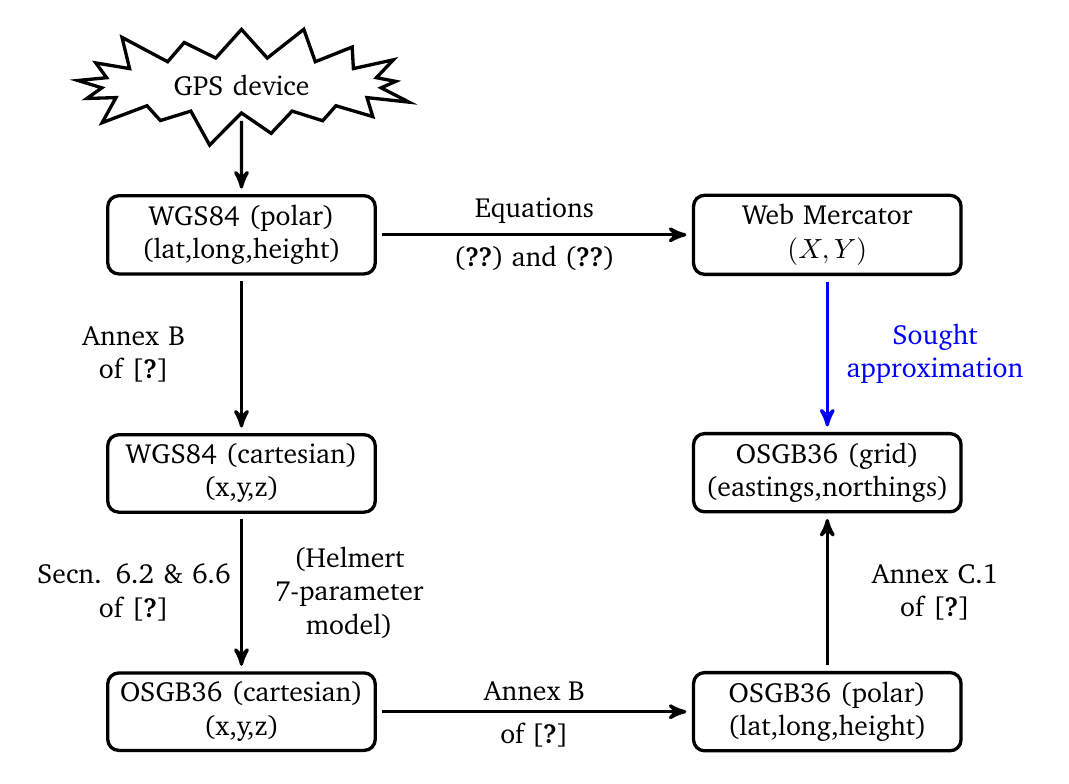
\begin{tikzpicture}
  \begin{scope}
  \node[box] (wgs84-polar) {WGS84 (polar) \linebreak (lat,long,height)};
  \node[box, right=4cm of wgs84-polar] (wm) {Web Mercator \linebreak $(X,Y)$};
  \node[box, below=2cm of wgs84-polar] (wgs84-xyz) {WGS84 (cartesian) \linebreak (x,y,z)};
  \node[box, below=2cm of wgs84-xyz] (osgb36-xyz) {OSGB36 (cartesian) \linebreak (x,y,z)};
  \node[box, right=4cm of osgb36-xyz] (osgb36-polar) {OSGB36 (polar) \linebreak (lat,long,height)};
  \node[box, above=2cm of osgb36-polar] (osgb36-en) {OSGB36 (grid) \linebreak (eastings,northings)};

  \path [arr,->] (wgs84-polar)
    edge
      node[above]{Equations}
      node[below]{\eqref{eqn:wmx} and \eqref{eqn:wmy}}
        (wm);

  \path [arr,->] (wgs84-polar)
    edge
      node[annot,left]{Annex B\\ of \cite{gcs}}
      (wgs84-xyz);

  \path [arr,->] (osgb36-xyz)
    edge
      node[above]{Annex B}
      node[below]{of \cite{gcs}}
      (osgb36-polar);

  \path [arr,->] (osgb36-polar)
    edge
      node[annot,right]{Annex C.1\\ of \cite{gcs}}
      (osgb36-en);

  \path [bluearr,->] (wm)
    edge
      node[annot,right,blue]{Sought\\approximation}
      (osgb36-en);

  \path [arr,->] (wgs84-xyz)
    edge node[annot,left]{Secn. 6.2 \& 6.6\\ of \cite{gcs}}
         node[annot,right]{(Helmert\\7-parameter\\model)}
    (osgb36-xyz);

  \node[boxzag, above=of wgs84-polar] ((gps) {GPS device}
    edge[arr,->] (wgs84-polar.north);

  \end{scope}
\end{tikzpicture}
\caption{The first approximation to eastings and northings}
\label{fig:derivation_helmert}

  \hrulefill
\end{figure}
% ----------------------------------------------------------------------------

Starting from WGS84 (lat,long) pairs that iterate over a region spanning the
UK, two transforms are applied, as illustrated in figure
\ref{fig:derivation_helmert}:

\begin{enumerate}
  \item from WGS84 to web mercator using equations \eqref{eqn:wmx} and \eqref{eqn:wmy}
  \item from WGS84 to OSGB36 lat,long using section 6.2 of \cite{gcs}, then
    from OSGB36 lat,lon to grid eastings,northings using annexe C1 of \cite{gcs}.
\end{enumerate}

Applying these two transforms to the WGS84 lat,long pairs provides a grid of
points over the UK, where each point is represented in two ways : as web
mercator X,Y and as grid reference E,N.

The goal was to find a reasonably simple model to approximate E,N from X,Y.
The first attempt was to fit a 2D power series by least squares.   As mentioned
earlier, the X and Y coordinates are transformed into $\alpha$, $\beta$ as
follows:

\begin{align}
  \alpha &= 61 (X-0.494440093) \label{eqn:alpha_X} \\
  \beta  &= 36 (Y-0.312663855) \label{eqn:beta_Y}
\end{align}

that is, by shifting them to an origin roughly in the middle of the UK and then
scaling them, so that the shifted + scaled coordinates like in the range
$[-1,+1]$ over the UK.  This makes it easy to see which terms in the power
series have negligible effect, and allows the method described in section
\ref{sec:reduction} to work.  The power series then take the form

\begin{align}
\hat{E} &= \sum_{i=0}^{N_\alpha - 1} \sum_{j=0}^{N_\beta - 1} e_{ij}\alpha^i\beta^j \\
\hat{N} &= \sum_{i=0}^{N_\alpha - 1} \sum_{j=0}^{N_\beta - 1} n_{ij}\alpha^i\beta^j \\
\end{align}

where $N_\alpha$ and $N_\beta$ define the order of the power series, $\hat{E}$
and $\hat{N}$ are the estimated eastings and northings, and $e_{ij}$, $n_{ij}$
are the sets of coefficients to be solved for.

To derive a solution for $e_{ij}$, $n_{ij}$ by least squares, a grid of $T$ points
$(\mu,\lambda)_n$ is selected in WGS84 space, where $\mu$ is latitude and
$\lambda$ is longitude.  $(X,Y)_n$ is calculated from this by equations
\eqref{eqn:wmx} and \eqref{eqn:wmy}, then $(\alpha,\beta)_n$ from $(X,Y)_n$ by
equations \eqref{eqn:alpha_X} and \eqref{eqn:beta_Y}.

For the initial model, we find $e_{ij}$, $n_{ij}$ that map $(X,Y)$ to eastings,
northings computed using the 7-parameter Helmert transform method.  Starting
from $(\mu,\lambda)_n$, the eastings, northings are computed as $(E,N)_n$.

Then the squared position error at each grid point $S^2_n$ is given by

\begin{align}
S^2_n = \left(E_n - \hat{E}_n\right)^2 + \left(N_n - \hat{N}_n\right)^2
\end{align}

The sum of squared errors is

\begin{align}
S^2 & = \sum_{n=1}^{T} S^2_n \\
    & = \sum_{n=1}^{T} \left(E_n - \hat{E}_n\right)^2 + \left(N_n - \hat{N}_n\right)^2
\end{align}

To simplify the process slightly, the eastings and northings are treated
separately, so we have two sum of squared errors $S^2_E$ and $S^2_N$ given by

\begin{align}
S^2_E & = \sum_{n=1}^{T} \left(E_n - \hat{E}_n\right)^2 \\
S^2_N & = \sum_{n=1}^{T} \left(N_n - \hat{N}_n\right)^2
\end{align}

Considering the eastings coefficients (the process is of course the same for
the northings),

\begin{align}
S^2_E & = \sum_{n=1}^{T} \left(E_n - \hat{E}_n\right)^2 \\
      & = \sum_{n=1}^{T} \left(E_n - 
   \sum_{i=0}^{N_\alpha - 1} \sum_{j=0}^{N_\beta - 1} e_{ij}\alpha^i_n\beta^j_n
   \right)^2
\end{align}

Then to form a set of equations to solve, take partial derivatives
against each $e_{uv}$ as follows:
\begin{align}
\frac{\partial S^2_E}{\partial e_{uv}} & =
  \sum_{n=1}^{T} 2 \left(E_n - 
   \sum_{i=0}^{N_\alpha - 1} \sum_{j=0}^{N_\beta - 1} e_{ij}\alpha^i_n\beta^j_n
   \right)
   \cdot
   \left(
     -\alpha_n^u \beta_n^v
   \right)
\intertext{Then setting}
   \frac{\partial S^2_E}{\partial e_{uv}} & = 0
\end{align}

for each $(u,v)$ pair, we have a set of $N_\alpha N_\beta$ equations in the
$N_\alpha N_\beta$ unknowns $e_{ij}$ as follows (where $(u,v)$ indexes the
equation):

\begin{align}
\left[
\sum_{i=0}^{N_\alpha - 1} \sum_{j=0}^{N_\beta - 1} \left[
  \sum_{n=1}^{T}
     \alpha^{i+u}_n\beta^{j+v}_n
  \right]
  e_{ij}
\right]
   &= 
\sum_{n=1}^{T} \alpha^u_n\beta^v_n E_n
\end{align}

or put another way this can be written as

\begin{align}
M E &= R_E
\intertext{where}
M(uv,ij) &= \left [
    \sum_{n=1}^{T}
       \alpha^{i+u}_n\beta^{j+v}_n
  \right] \\
  E(ij) &= \left[ e_{ij} \right] \\
  R_E (uv) &= \left[
    \sum_{n=1}^{T} \alpha^u_n\beta^v_n E_n
  \right]
\end{align}

$ij$ and $uv$ each represent the 2D pair of indices, with some arbitrary
linearisation of the 2D set of equations and unknowns into a 1D arrangement.
For example, the linearisation might be

\begin{align}
  (u,v) & \mapsto u + vN_\alpha \\
  (i,j) & \mapsto i + jN_\alpha \\
  (i+u,j+v) & \mapsto (i + u) + (j + v)N_\alpha
\end{align}

The same procedure can be applied to the northings, giving

\begin{align}
\left[
\sum_{i=0}^{N_\alpha - 1} \sum_{j=0}^{N_\beta - 1} \left[
  \sum_{n=1}^{T}
     \alpha^{i+u}_n\beta^{j+v}_n
  \right]
  n_{ij}
\right]
   &= 
\sum_{n=1}^{T} \alpha^u_n\beta^v_n N_n
\intertext{or}
M N &= R_N
\intertext{where}
M(uv,ij) &= \left [
    \sum_{n=1}^{T}
       \alpha^{i+u}_n\beta^{j+v}_n
  \right] \\
  N(ij) &= \left[ n_{ij} \right] \\
  R_N (uv) &= \left[
    \sum_{n=1}^{T} \alpha^u_n\beta^v_n N_n
  \right]
\end{align}

the matrix $M$ is the same in each case.  These linear equations can be solved
by any standard method such as Gaussian elimination.

Power series of degree 3 or less in both variables (i.e. up to 16 terms)
provided a useless approximation and clearly did not have enough terms for the
model to fit the shape of the stretched rectangle inherent in the OS projection
(see figure 8 of \cite{gcs}, figure \ref{fig:grid_wm} of this paper).  The
equations were solved for terms up to $\alpha^5\beta^v$ and $\alpha^u\beta^5$
(i.e. 36 coefficients in total).  Many of the resulting coefficients are
negligible, with magnitudes much less than 1, as is seen in table
\ref{tbl:raw_lsq_helmert} below.

% ----------------------------------------------------------------------------
\begin{table}
  \centering
\begin{tabular}{l l r r}
\toprule
\textbf{i} & \textbf{j} & $e_{ij}$ & $n_{ij}$ \\
\midrule
0 & 0 &    400000.02304 &    650000.01926 \\
0 & 1 &       -16.51336 &   -626485.24808 \\
0 & 2 &        -0.65620 &    -44898.45338 \\
0 & 3 &         0.07299 &     -1115.85828 \\
0 & 4 &         0.01262 &       107.47381 \\
0 & 5 &         0.00051 &        13.94758 \\
1 & 0 &    370518.52837 &        -9.75573 \\
1 & 1 &     53335.51178 &        -0.79381 \\
1 & 2 &      2037.81039 &         0.10263 \\
1 & 3 &      -247.15294 &         0.03678 \\
1 & 4 &       -41.68524 &        -0.00896 \\
1 & 5 &        -2.37372 &         0.03627 \\
2 & 0 &         0.23444 &     15771.95616 \\
2 & 1 &        -0.07511 &      1215.27474 \\
2 & 2 &        -0.04408 &      -217.30648 \\
2 & 3 &         0.01434 &       -51.19676 \\
2 & 4 &        -0.00377 &        -3.43000 \\
2 & 5 &         0.00336 &         1.37746 \\
\bottomrule
\end{tabular}
\quad\quad
\begin{tabular}{l l r r}
\toprule
\textbf{i} & \textbf{j} & $e_{ij}$ & $n_{ij}$ \\
\midrule
3 & 0 &      -239.52751 &        -0.07786 \\
3 & 1 &        85.62368 &         0.38050 \\
3 & 2 &        29.43609 &        -0.38243 \\
3 & 3 &         2.59671 &        -0.60514 \\
3 & 4 &        -0.32301 &         1.22739 \\
3 & 5 &         0.26406 &        -0.55790 \\
4 & 0 &        -0.02455 &        12.45049 \\
4 & 1 &         0.06190 &         8.51989 \\
4 & 2 &         0.11854 &         2.35361 \\
4 & 3 &        -0.33542 &         1.28934 \\
4 & 4 &         0.12723 &        -4.07999 \\
4 & 5 &         0.05574 &         1.88473 \\
5 & 0 &        -1.03817 &        -0.11168 \\
5 & 1 &        -0.28302 &        -0.20765 \\
5 & 2 &         0.02942 &         1.42322 \\
5 & 3 &        -0.02110 &         0.32854 \\
5 & 4 &         0.27261 &        -4.80810 \\
5 & 5 &        -0.24941 &         3.40551 \\
\bottomrule
\end{tabular}
\caption{$e_{ij}$ and $n_{ij}$ from the least squares solution to the 7-parameter model}
\label{tbl:raw_lsq_helmert}
\hrulefill
\end{table}

% ----------------------------------------------------------------------------
After applying the method of section \ref{sec:reduction} to prune all
insignificant coefficients, using a tolerance of no more than 1 metre of
additional errors being introduced, these formulae remain:
\begin{align}
E_0 &= 400000.17 -16.55\beta -0.67\beta^2\nonumber \\
E_1 &= 370518.85 +53336.32\beta +2037.80\beta^2 -250.02\beta^3 -41.77\beta^4\nonumber \\
E_3 &= -240.83 +85.28\beta +29.49\beta^2 +2.51\beta^3\nonumber \\
E &= E_0 +E_1\alpha +E_3\alpha^3
  \label{eqn:untrimmed_east}
\\[1ex]
N_0 &= 650000.02 -626485.25\beta -44898.45\beta^2 -1115.86\beta^3 +107.47\beta^4 +13.95\beta^5\nonumber \\
N_1 &= -10.17 -0.53\beta\nonumber \\
N_2 &= 15771.96 +1214.84\beta -217.31\beta^2 -49.47\beta^3 -3.43\beta^4\nonumber \\
N_3 &= 2.62\beta^2 -0.89\beta^3\nonumber \\
N_4 &= 12.45 +7.93\beta +2.35\beta^2 +3.65\beta^3 -4.08\beta^4\nonumber \\
N_5 &= -4.81\beta^4 +3.41\beta^5\nonumber \\
N &= N_0 +N_1\alpha +N_2\alpha^2 +N_3\alpha^3 +N_4\alpha^4 +N_5\alpha^5
  \label{eqn:untrimmed_north}
\end{align}

Figure \ref{fig:untrimmed_v_7param} shows the modelling error (in metres) ---
showing that the terms in the equations are of sufficiently high order to give
a good model of the `long' route in figure \ref{fig:derivation_helmert}.

\subsection{Comparing the initial model with OSTN02}

If the model of equations \eqref{eqn:untrimmed_east} and
\eqref{eqn:untrimmed_north} is compared against the OSTN02 model, the error is
as shown in figure \ref{fig:untrimmed_v_ostn02}.  The procedure for applying
the OSTN02 model is shown in figure \ref{fig:derivation_ostn02}.  In this
figure, the red arrow shows the final approximation that is sought.  The blue
arrow shows the approximation of equations \eqref{eqn:untrimmed_east} and
\eqref{eqn:untrimmed_north} earlier, and the purple arrow shows the error
between the two (figure \ref{fig:untrimmed_v_ostn02}).  In other words,
equations \eqref{eqn:untrimmed_east} and \eqref{eqn:untrimmed_north} are a good
model for figure \ref{fig:derivation_helmert}.

% ----------------------------------------------------------------------------
\begin{figure}[htbp]
  \hrulefill

  \centering
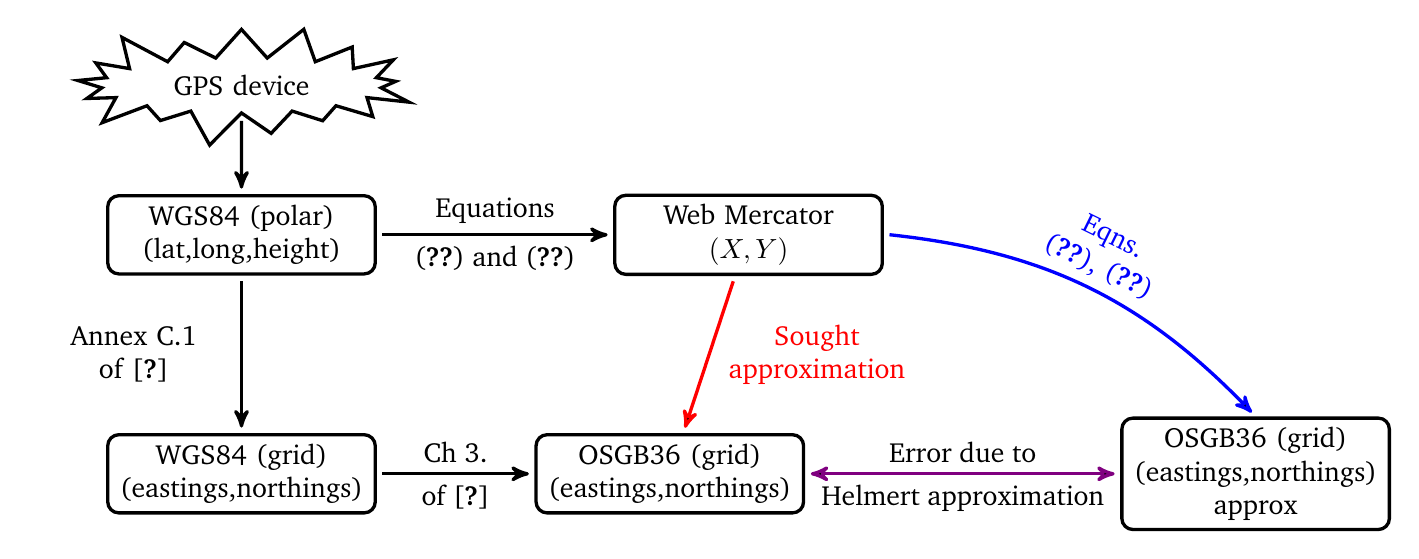
\begin{tikzpicture}
  \begin{scope}
  \node[box] (wgs84-polar) {WGS84 (polar) \linebreak (lat,long,height)};
  \node[box, right=3cm of wgs84-polar] (wm) {Web Mercator \linebreak $(X,Y)$};
  \node[box, below=2cm of wgs84-polar] (wgs84-en) {WGS84 (grid) \linebreak (eastings,northings)};
  \node[box, right=2cm of wgs84-en] (osgb36-en) {OSGB36 (grid) \linebreak (eastings,northings)};
  \node[box, right=4cm of osgb36-en] (osgb36-en-a) {OSGB36 (grid) \linebreak (eastings,northings)\\approx};

  \path [arr,->] (wgs84-polar)
    edge
      node[above]{Equations}
      node[below]{\eqref{eqn:wmx} and \eqref{eqn:wmy}}
        (wm);

  \path [arr,->] (wgs84-polar)
    edge
      node[annot,left]{Annex C.1\\of \cite{gcs}}
      (wgs84-en);

  \path [arr,->] (wgs84-en)
    edge
      node[above]{Ch 3.}
      node[below]{of \cite{toug}}
      (osgb36-en);

  \path [bluearr,->,bend left=20] (wm)
    edge
      node[annot,sloped,above,blue]{Eqns. \eqref{eqn:untrimmed_east}, \eqref{eqn:untrimmed_north}}
      (osgb36-en-a.north);

  \path [purparr,<->] (osgb36-en)
    edge
      node[above]{Error due to}
      node[below]{Helmert approximation}
    (osgb36-en-a);

  \path [redarr,->] (wm)
    edge
      node[annot,right,red]{Sought\\approximation}
      (osgb36-en);

  \node[boxzag, above=of wgs84-polar] ((gps) {GPS device}
    edge[arr,->] (wgs84-polar.north);

  \end{scope}
\end{tikzpicture}
\caption{The accurate calculation for grid eastings and northings}
\label{fig:derivation_ostn02}

  \hrulefill
\end{figure}
% ----------------------------------------------------------------------------

\begin{figure}[htb]
  \begin{subfigure}[b]{0.4\textwidth}
  \centering
  \fbox{
    \input wm_to_grid_notrim_7param.tex
  }
  \caption{against the original 7-parameter model}
  \label{fig:untrimmed_v_7param}
\end{subfigure}
\gap
  \begin{subfigure}[b]{0.4\textwidth}
  \centering
  \fbox{
    \input wm_to_grid_notrim_ostn.tex
  }
  \caption{against OSTN02}
  \label{fig:untrimmed_v_ostn02}
\end{subfigure}
  \caption{Positional errors (in metres) using \eqref{eqn:untrimmed_east} and \eqref{eqn:untrimmed_north}}
\hrulefill
\end{figure}

The remaining problem is that the OSGB36 eastings, northings calculated
according to figure \ref{fig:derivation_helmert} are \textbf{not} the same as
those calculated by the OSTN02 model shown in figure
\ref{fig:derivation_ostn02}, and this is the source of the error shown in
figure \ref{fig:untrimmed_v_ostn02}.

\subsection{Adjusting the model to represent OSTN02 better}

The `obvious' solution to this is to do the least-squares fit, but using the
OSTN02 position directly as the target function in place of the position
estimated by the 7-parameter model.

This approach was in fact tried.  The resulting $e_{ij}$, $n_{ij}$ coefficients
had many terms of large magnitude.  This suggested that the behaviour was
somewhat unstable and offered little opportunity for thinning out the number of
active terms.  If the order of the polynomials was increased, the situation did
not improve.  The OSTN02 model contains a lot of localised but small variation
and a high-order polynomial tried `too hard' to follow these sub-metre
variations.

On the other hand, a polynomial up to order 4 or 5 in both directions is
necessary to match the macroscopic behaviour --- as found by the least-squares
fit to the 7-parameter model in section \ref{sec:lsq_helmert}.

This conflict implies it is impossible to aim directly for a least-squares
model of OSTN02.  However, the difference between the 7-parameter model and
OSTN02 has already been shown, in figure \ref{fig:untrimmed_v_ostn02}.  If
\textbf{this} error function is modelled by a separate least-squares fit, using
relatively low order polynomials to provide smoothing instead of
`over-modelling', the resulting coefficients can be added to those from the
7-parameter model earlier to give a result that fits OSTN02 much more closely.

The trimming coefficients are shown in table \ref{tbl:trim_helmert_ostn02}.
These are added to the matching subset of coefficients in table
\ref{tbl:raw_lsq_helmert}, and the resulting set reduced by the method of
section \ref{sec:reduction}.  Finally this yields the formulae shown earlier in
equations \eqref{eqn:east1} and \eqref{eqn:north1}.

% ----------------------------------------------------------------------------
\begin{table}
  \centering
\begin{tabular}{l l r r}
\toprule
\textbf{i} & \textbf{j} & $\Delta{}e_{ij}$ & $\Delta{}n_{ij}$ \\
\midrule
0 & 0 &         0.67265 &        -0.07365 \\
0 & 1 &        -1.04003 &        -5.82258 \\
0 & 2 &        -1.06955 &         0.12794 \\
0 & 3 &         0.54481 &        10.60766 \\
1 & 0 &         4.52788 &        -1.83891 \\
1 & 1 &        -9.39493 &         0.33639 \\
1 & 2 &       -12.11921 &         5.04263 \\
1 & 3 &         8.74946 &        -3.18270 \\
\bottomrule
\end{tabular}
\quad\quad
\begin{tabular}{l l r r}
\toprule
\textbf{i} & \textbf{j} & $\Delta{}e_{ij}$ & $\Delta{}n_{ij}$ \\
\midrule
2 & 0 &         3.08354 &        -2.96744 \\
2 & 1 &       -18.96895 &        -2.10783 \\
2 & 2 &        14.64681 &         5.24938 \\
2 & 3 &        10.64015 &        -3.76395 \\
3 & 0 &         3.14420 &        -3.25315 \\
3 & 1 &        -7.44719 &         4.76809 \\
3 & 2 &        11.71811 &         8.47039 \\
3 & 3 &         4.23068 &        -5.70590 \\
\bottomrule
\end{tabular}
\caption{Adjustments to apply to $e_{ij}$ and $n_{ij}$ to account for the difference between the 7-parameter model and the OSTN02 model}
\label{tbl:trim_helmert_ostn02}
\hrulefill
\end{table}
% ----------------------------------------------------------------------------

\subsection{Term reduction}
\label{sec:reduction}
The least squares model described earlier produces a significant number of
negligible coefficients --- those which contribute at most a few centimetres to
the position.  A method was sought to allow terms to be dropped from the power
series subject to staying within a pre-defined error budget.  To ease
computational cost, terms with higher powers of $\alpha$ and $\beta$ are to be
dropped first if possible.

The method used relies on Chebyshev polynomials of the first kind.  These are defined by

\begin{align}
  T_0(x) & = 1 \\
  T_1(x) &= x \\
  T_n(x) &= 2xT_{n-1}(x) - T_{n-2}(x)
\end{align}

and have the property that for $x \in [-1,1]$, $T_n(x) \in [-1,1]$ for all $n$.

For example,
\begin{align}
  T_5(x) = 16x^5 - 20x^3 + 5x
\end{align}

Because $T_5(x) \in [-1,1]$, we can approximate $x^5$ over the range $[-1,1]$ by

\begin{align}
  x^5 \approx \frac{20x^3}{16} - \frac{5x}{16}
\end{align}

where the approximation error $\epsilon$ is given by $|\epsilon| <
\frac{1}{16}$.  Because of the power-of-two effect, high-order terms are the
easiest to remove from the formulae.  This is convenient because they are the
more expensive terms to calculate in the phone at runtime due to the extra
multiplications.

If the terms in the formulae earlier are written $c_{ij}\alpha^i\beta^j$,
suppose $i<j$.  Then calculate $\epsilon_{ij} = |c_{ij}|2^{-(j-1)}$.  If $i\ge j$
compute $\epsilon_{ij} = |c_{ij}|2^{-(i-1)}$.
For terms where $i$ and $j$ are both less than 2, we take $\epsilon_{ij} =
|c_{ij}|$ because the term will be discarded rather than replaced with
lower-order terms.
Then find $i,j$ such that $\epsilon_{ij}$ has the smallest magnitude over all
terms for which $c_{ij} \ne 0$.  Assuming $\epsilon_{ij}$ is not too large, the
$\alpha^i\beta^j$ term is replaced by 0 and the appropriate lower-order
coefficients are adjusted according to the coefficients in the appropriate
Chebyshev polynomial, scaled according to the value of $c_{ij}$ being replaced.

The criterial for `largeness' is to keep a total of all $\epsilon_{ij}$ values
so far, and check whether adding the next term will cross a threshold value.
The threshold value is chosen according to the accuracy required in the
remaining formula.  The threshold value is typically larger than the required
accuracy, because the approximation errors caused by dropping terms do not all
have the same sign in any one location, so tend to partially cancel one another
out.  A suitable threshold is found by trial and error.

\section {From grid references to Web Mercator}
It is also useful to be able to start from a grid reference $(E,N)$ (assumed
all-numeric here) and compute the equivalent Web Mercator coordinates $(X,Y)$.
Given these, it is simple to get the latitude $M$ and longitude $L$ (in
\textbf{radians}) by

\begin{align}
  L &= (2X - 1)\pi \\
  M &= \left[2\tan^{-1}\left(e^t\right)\right] - \frac{\pi}{2} \\
  \label{eqn:y_to_M}
  \intertext{where}
  t &= (1 - 2Y)\pi
\end{align}

The latitude formula uses the Gudermannian function.

Given the all-numeric (6-figure) eastings, northings $(E,N)$, let

\begin{align}
  \eta &= \frac{E - 400000}{400000} \\[1ex]
  \nu  &= \frac{N - 650000}{650000}
\end{align}

As in the earlier sections, the shifting and scaling are to bring $\eta, \nu$
both into the range $[-1,1]$ over the defined range of grid coordinates.
Similarly, in the following formulae, the coefficients are scaled so that they
represent approximately metres at the edges of the grid, which makes it much
easier to determine which terms are negligible.

A two-stage least-squares fitting process similar to that used earlier was used
to generate the following models from $(\eta,\nu) \mapsto (X,Y)$.

The following formulae will calculate $(X,Y)$ accurate to under a metre across
GB, as shown in figure \ref{fig:grid_to_wm_1m}:
\begin{align}
X_0 &= 12361001.62 -19.66\nu -2.24\nu^2\nonumber \\
X_1 &= 442441.04 +66066.30\nu +12171.89\nu^2 +2057.38\nu^3 +364.45\nu^4 +62.11\nu^5\nonumber \\
X_2 &= -2.52 -23.19\nu -23.76\nu^2 +3.72\nu^3\nonumber \\
X_3 &= -1540.23 -778.77\nu -273.35\nu^2 -63.49\nu^3 -25.26\nu^4 -12.21\nu^5\nonumber \\
X_4 &= 7.76\nu^3 +6.93\nu^4\nonumber \\
X_5 &= 10.01 +12.09\nu^4 +10.61\nu^5\nonumber \\
25000000 X &= X_0 +X_1\eta +X_2\eta^2 +X_3\eta^3 +X_4\eta^4 +X_5\eta^5
  \label{eqn:x1}
\\[1ex]
Y_0 &= 7816596.43 -720504.09\nu -53575.89\nu^2 -6596.44\nu^3 -830.91\nu^4 -117.01\nu^5 -15.94\nu^6\nonumber \\
Y_1 &= -13.88 -5.83\nu +4.10\nu^2 +4.32\nu^3\nonumber \\
Y_2 &= 20368.69 +7485.47\nu +1909.20\nu^2 +454.99\nu^3 +98.62\nu^4 +23.58\nu^5\nonumber \\
Y_3 &= -9.34 -12.10\nu +26.34\nu^2 +23.54\nu^3 -5.75\nu^4\nonumber \\
Y_4 &= -119.10 -84.19\nu -41.68\nu^2 -7.53\nu^3 +20.95\nu^4 +15.10\nu^5\nonumber \\
Y_5 &= 14.47\nu^4 +30.69\nu^5 +14.37\nu^6\nonumber \\
25000000 Y &= Y_0 +Y_1\eta +Y_2\eta^2 +Y_3\eta^3 +Y_4\eta^4 +Y_5\eta^5
  \label{eqn:y1}
\end{align}

\begin{figure}[htb]
  \begin{subfigure}[b]{0.4\textwidth}
  \centering
  \fbox{
    \input grid_to_wm_1m.tex
  }
  \caption{achieved using equations \eqref{eqn:x1} and \eqref{eqn:y1}}
  \label{fig:grid_to_wm_1m}
\end{subfigure}
\gap
  \begin{subfigure}[b]{0.4\textwidth}
  \centering
  \fbox{
    \input grid_to_wm_10m.tex
  }
  \caption{achieved using equations \eqref{eqn:x10} and \eqref{eqn:y10}}
  \label{fig:grid_to_wm_10m}
\end{subfigure}
  \caption{Positional error (in metres against OSTN02)}
\hrulefill
\end{figure}

There are significantly more active terms in this expression than in the $(X,Y)
\mapsto (E, N)$ direction.  The reason is not apparent.  A coarser model
with fewer terms is given by equations \eqref{eqn:x10} and \eqref{eqn:y10}.
The error, below 10m across GB, is shown in figure \ref{fig:grid_to_wm_10m}.

\begin{align}
X_0 &= 12360998.48 -27.68\nu\nonumber \\
X_1 &= 442437.92 +66047.92\nu +12171.89\nu^2 +2130.87\nu^3 +360.67\nu^4\nonumber \\
X_2 &= -16.83\nu^2\nonumber \\
X_3 &= -1526.46 -779.10\nu -283.50\nu^2 -62.17\nu^3\nonumber \\
25000000 X &= X_0 +X_1\eta +X_2\eta^2 +X_3\eta^3
  \label{eqn:x10}
\\[1ex]
Y_0 &= 7816595.94 -720504.09\nu -53564.33\nu^2 -6597.86\nu^3 -854.82\nu^4 -117.01\nu^5\nonumber \\
Y_1 &= -20.97 -8.99\nu\nonumber \\
Y_2 &= 20368.69 +7478.10\nu +1888.46\nu^2 +495.81\nu^3 +98.62\nu^4\nonumber \\
Y_3 &= -24.09\nu +10.49\nu^2 +71.49\nu^3 +45.02\nu^4\nonumber \\
Y_4 &= -121.72 -88.91\nu\nonumber \\
25000000 Y &= Y_0 +Y_1\eta +Y_2\eta^2 +Y_3\eta^3 +Y_4\eta^4
  \label{eqn:y10}
\end{align}

\section {Contour key}
\begin{table}[h]
\centering
\begin{tabular}{r l}
\toprule
\textbf{Level} & \textbf{Sample} \\
\midrule
0.00 & {\tikz \draw [black,thick] (0cm,1ex) node[fill=white,fill opacity=0.7,text opacity=1,font=\tiny,text=black,inner sep=1pt,draw=black,thin,draw opacity=1] {0.00}-- ++(1cm,0cm);}\\
0.10 & {\tikz \draw [purple!70!blue!80!white,thin] (0cm,1ex) node[fill=white,fill opacity=0.7,text opacity=1,font=\tiny,text=purple!70!blue!80!white,inner sep=1pt,draw=purple!70!blue!80!white,thin,draw opacity=1] {0.10}-- ++(1cm,0cm);}\\
0.13 & {\tikz \draw [blue,thin] (0cm,1ex) node[fill=white,fill opacity=0.7,text opacity=1,font=\tiny,text=blue,inner sep=1pt,draw=blue,thin,draw opacity=1] {0.13}-- ++(1cm,0cm);}\\
0.18 & {\tikz \draw [cyan!90!black,thin] (0cm,1ex) node[fill=white,fill opacity=0.7,text opacity=1,font=\tiny,text=cyan!90!black,inner sep=1pt,draw=cyan!90!black,thin,draw opacity=1] {0.18}-- ++(1cm,0cm);}\\
0.25 & {\tikz \draw [green!70!black,thin] (0cm,1ex) node[fill=white,fill opacity=0.7,text opacity=1,font=\tiny,text=green!70!black,inner sep=1pt,draw=green!70!black,thin,draw opacity=1] {0.25}-- ++(1cm,0cm);}\\
0.35 & {\tikz \draw [yellow!95!red!70!black,thin] (0cm,1ex) node[fill=white,fill opacity=0.7,text opacity=1,font=\tiny,text=yellow!95!red!70!black,inner sep=1pt,draw=yellow!95!red!70!black,thin,draw opacity=1] {0.35}-- ++(1cm,0cm);}\\
0.50 & {\tikz \draw [orange!80!black,thin] (0cm,1ex) node[fill=white,fill opacity=0.7,text opacity=1,font=\tiny,text=orange!80!black,inner sep=1pt,draw=orange!80!black,thin,draw opacity=1] {0.50}-- ++(1cm,0cm);}\\
\bottomrule
\end{tabular}
\quad
\begin{tabular}{r l}
\toprule
\textbf{Level} & \textbf{Sample} \\
\midrule
0.70 & {\tikz \draw [red,thin] (0cm,1ex) node[fill=white,fill opacity=0.7,text opacity=1,font=\tiny,text=red,inner sep=1pt,draw=red,thin,draw opacity=1] {0.70}-- ++(1cm,0cm);}\\
1.00 & {\tikz \draw [purple!70!blue!80!white,thick] (0cm,1ex) node[fill=white,fill opacity=0.7,text opacity=1,font=\tiny,text=purple!70!blue!80!white,inner sep=1pt,draw=purple!70!blue!80!white,thin,draw opacity=1] {1.0}-- ++(1cm,0cm);}\\
1.30 & {\tikz \draw [blue,thick] (0cm,1ex) node[fill=white,fill opacity=0.7,text opacity=1,font=\tiny,text=blue,inner sep=1pt,draw=blue,thin,draw opacity=1] {1.3}-- ++(1cm,0cm);}\\
1.80 & {\tikz \draw [cyan!90!black,thick] (0cm,1ex) node[fill=white,fill opacity=0.7,text opacity=1,font=\tiny,text=cyan!90!black,inner sep=1pt,draw=cyan!90!black,thin,draw opacity=1] {1.8}-- ++(1cm,0cm);}\\
2.50 & {\tikz \draw [green!70!black,thick] (0cm,1ex) node[fill=white,fill opacity=0.7,text opacity=1,font=\tiny,text=green!70!black,inner sep=1pt,draw=green!70!black,thin,draw opacity=1] {2.5}-- ++(1cm,0cm);}\\
3.50 & {\tikz \draw [yellow!95!red!70!black,thick] (0cm,1ex) node[fill=white,fill opacity=0.7,text opacity=1,font=\tiny,text=yellow!95!red!70!black,inner sep=1pt,draw=yellow!95!red!70!black,thin,draw opacity=1] {3.5}-- ++(1cm,0cm);}\\
5.00 & {\tikz \draw [orange!80!black,thick] (0cm,1ex) node[fill=white,fill opacity=0.7,text opacity=1,font=\tiny,text=orange!80!black,inner sep=1pt,draw=orange!80!black,thin,draw opacity=1] {5.0}-- ++(1cm,0cm);}\\
\bottomrule
\end{tabular}
\quad
\begin{tabular}{r l}
\toprule
\textbf{Level} & \textbf{Sample} \\
\midrule
7.00 & {\tikz \draw [red,thick] (0cm,1ex) node[fill=white,fill opacity=0.7,text opacity=1,font=\tiny,text=red,inner sep=1pt,draw=red,thin,draw opacity=1] {7.0}-- ++(1cm,0cm);}\\
10.00 & {\tikz \draw [purple!70!blue!80!white,very thick] (0cm,1ex) node[fill=white,fill opacity=0.7,text opacity=1,font=\tiny,text=purple!70!blue!80!white,inner sep=1pt,draw=purple!70!blue!80!white,thin,draw opacity=1] {10}-- ++(1cm,0cm);}\\
13.00 & {\tikz \draw [blue,very thick] (0cm,1ex) node[fill=white,fill opacity=0.7,text opacity=1,font=\tiny,text=blue,inner sep=1pt,draw=blue,thin,draw opacity=1] {13}-- ++(1cm,0cm);}\\
18.00 & {\tikz \draw [cyan!90!black,very thick] (0cm,1ex) node[fill=white,fill opacity=0.7,text opacity=1,font=\tiny,text=cyan!90!black,inner sep=1pt,draw=cyan!90!black,thin,draw opacity=1] {18}-- ++(1cm,0cm);}\\
25.00 & {\tikz \draw [green!70!black,very thick] (0cm,1ex) node[fill=white,fill opacity=0.7,text opacity=1,font=\tiny,text=green!70!black,inner sep=1pt,draw=green!70!black,thin,draw opacity=1] {25}-- ++(1cm,0cm);}\\
35.00 & {\tikz \draw [yellow!95!red!70!black,very thick] (0cm,1ex) node[fill=white,fill opacity=0.7,text opacity=1,font=\tiny,text=yellow!95!red!70!black,inner sep=1pt,draw=yellow!95!red!70!black,thin,draw opacity=1] {35}-- ++(1cm,0cm);}\\
50.00 & {\tikz \draw [orange!80!black,very thick] (0cm,1ex) node[fill=white,fill opacity=0.7,text opacity=1,font=\tiny,text=orange!80!black,inner sep=1pt,draw=orange!80!black,thin,draw opacity=1] {50}-- ++(1cm,0cm);}\\
\bottomrule
\end{tabular}
\quad
\begin{tabular}{r l}
\toprule
\textbf{Level} & \textbf{Sample} \\
\midrule
70.00 & {\tikz \draw [red,very thick] (0cm,1ex) node[fill=white,fill opacity=0.7,text opacity=1,font=\tiny,text=red,inner sep=1pt,draw=red,thin,draw opacity=1] {70}-- ++(1cm,0cm);}\\
100.00 & {\tikz \draw [purple!70!blue!80!white,ultra thick] (0cm,1ex) node[fill=white,fill opacity=0.7,text opacity=1,font=\tiny,text=purple!70!blue!80!white,inner sep=1pt,draw=purple!70!blue!80!white,thin,draw opacity=1] {100}-- ++(1cm,0cm);}\\
130.00 & {\tikz \draw [blue,ultra thick] (0cm,1ex) node[fill=white,fill opacity=0.7,text opacity=1,font=\tiny,text=blue,inner sep=1pt,draw=blue,thin,draw opacity=1] {130}-- ++(1cm,0cm);}\\
180.00 & {\tikz \draw [cyan!90!black,ultra thick] (0cm,1ex) node[fill=white,fill opacity=0.7,text opacity=1,font=\tiny,text=cyan!90!black,inner sep=1pt,draw=cyan!90!black,thin,draw opacity=1] {180}-- ++(1cm,0cm);}\\
250.00 & {\tikz \draw [green!70!black,ultra thick] (0cm,1ex) node[fill=white,fill opacity=0.7,text opacity=1,font=\tiny,text=green!70!black,inner sep=1pt,draw=green!70!black,thin,draw opacity=1] {250}-- ++(1cm,0cm);}\\
\bottomrule
\end{tabular}
\caption{Key to the contour levels in the maps}
\label{tbl:contour_key}
\hrulefill
\end{table}

\section {Worked example}
This section uses the Caister Water Tower example from appendix A of
\cite{toug}.  The ETRS89 location is given as 52\degree{}39'28.8282''N,
1\degree{}42'57.8663''E, 108.05m.

Applying first equation \eqref{eqn:ahat}, the ODN height is estimated as
64.64m.  The answer quoted in \cite{toug} is 63.806m.  The error is about 0.8m.

Then applying equations \eqref{eqn:east1} and \eqref{eqn:north1}, the eastings
and northings are estimated as E=651409.96, N=313177.58.  The correct values
quoted in \cite{toug} are E=651409.792, N=313177.448.  The errors are 17cm,
14cm respectively.

Taking now the OS-quoted eastings and northings and applying equations
\eqref{eqn:x1} and \eqref{eqn:y1} followed by equation \eqref{eqn:y_to_M}, the
latitude and longitude are estimated as 52.6580083,  1.7160707
respectively.  These have errors of approximately 4-microdegrees in latitude and
3 in longitude.  At the latitude of the UK, a degree of longitude is about
70km, so these errors are about 28cm, 21cm respectively.

\section {OS standard methods}
\label{sec:os_models}

In this section, the formulae used in the coordinate conversions of figure
\ref{fig:derivation_helmert} are described.

\paragraph{Polar to cartesian conversion}
\label{sec:polar_to_cart}
Assuming a position given by latitude $M$, longitude $L$, height above
ellipsoid $H$, and parameters semi major and minor axes of the WGS84 ellipsoid
$a$ and $b$ given in metres by $a = 6378137.0$, $b = 6356752.3141$.  Then proceed as follows (where $e$ is the eccentricity of the ellipsoid):

\begin{align}
  e^2 & = \left(1 - \dfrac{b^2}{a^2}\right) \\[2ex]
  \nu & = \frac{a}{\sqrt{1 - e^2 \sin^2{M}}} \\
  \intertext{then the cartesian coordinates are (see annex B.1 of \cite{gcs})}
x & = (\nu + H) \cos{M} \cos{L}
\label{eqn:ptoc_x} \\
y & = (\nu + H) \cos{M} \sin{L} \\
z & = \left(\left(1 - e^2\right)\nu + H\right)\sin{M}
\label{eqn:ptoc_z}
\end{align}

\paragraph{WGS84 to OSGB36 approximation}

The \textit{Helmert transform}, which is claimed in \cite{gcs} to give better
than 5 metre accuracy in the UK, is given by

\begin{equation}
  \left[ \begin{matrix}
    x \\ y \\ z
  \end{matrix}\right]_{OSGB36-like}
  =
  \left[ \begin{matrix}
    t_x \\ t_y \\ t_z
  \end{matrix}\right]
    +
  \left[ \begin{matrix}
      1+s & -r_z & r_y \\
      r_z & 1+s & -r_x \\
      -r_y & r_x  & 1+s
  \end{matrix}\right]
  \left[ \begin{matrix}
    x \\ y \\ z
  \end{matrix}\right]_{WGS84}
  \label{eqn:ctoc}
\end{equation}

where $t_x$, $t_y$, $t_z$ are a translation, $r_x$, $r_y$ and $r_z$ represent
a rotation, and $s$ is a scaling factor.  The values of these 7 parameters
are listed in section 6.6 of \cite{gcs}.  Equation \eqref{eqn:ctoc} is from
section 6.2 of \cite{gcs}.

\paragraph{Cartesian to polar conversion (in OSGB36)}
This is the inverse of the conversion shown in equations \eqref{eqn:ptoc_x}
through \eqref{eqn:ptoc_z}, but using different constants for $a$ and $b$
corresponding to the Airy 1830 ellipsoid.  It involves an iterative procedure
to solve for the latitude.  See annex B.2 of \cite{gcs}.

\paragraph{OSGB36 polar coordinates to national grid eastings and northings}
The formulae for these are in annex C.1 of \cite{gcs}.  They implement a
transverse Mercator projection and are relatively complicated.  They include
the $\sin$, $\cos$ and $\tan$ (and their powers) for several angles, as well as
taking square roots.  The reader is directed to \cite{gcs}.

\section {Implementation}
This section considers an implementation of equations \eqref{eqn:east1} and
\eqref{eqn:north1}.  If the target machine has a fused multiply-accumulate
instruction, the following representation may be attractive:
\begin{quote}
\small
\begin{verbatim}
double t0, t1, t2, t3, t4, t5, t6, t7;
double t8, t9, t10, t11, t12, t13;
double t14, t15, t16, t17, t18, t19, t20, t21;
double t22, t23, t24, t25, t26, t27, t28, t29;
double t30, t31, t32, t33, t34, t35;
double alpha2 = alpha * alpha;
double alpha4 = alpha2 * alpha2;
double beta2 = beta * beta;
double beta4 = beta2 * beta2;
t0 = (400000.70) + (-17.07)*beta;
t1 = t0 + (-1.74)*beta2;
t2 = (370523.38) + (53326.92)*beta;
t3 = (2025.68) + (-241.27)*beta;
t4 = t2 + t3*beta2;
t5 = t4 + (-41.77)*beta4;
t6 = t1 + t5*alpha;
t7 = (3.28) + (-19.00)*beta;
t8 = (14.84) + (10.39)*beta;
t9 = t7 + t8*beta2;
t10 = (-237.68) + (77.84)*beta;
t11 = (41.21) + (6.74)*beta;
t12 = t10 + t11*beta2;
t13 = t9 + t12*alpha;
E = t6 + t13*alpha2;
t14 = (649999.95) + (-626491.07)*beta;
t15 = (-44898.33) + (-1105.25)*beta;
t16 = t14 + t15*beta2;
t17 = (107.47) + (13.95)*beta;
t18 = t16 + t17*beta4;
t19 = (4.69) + (-4.53)*beta;
t20 = (-11.56) + t19*beta2;
t21 = t18 + t20*alpha;
t22 = (15768.99) + (1212.74)*beta;
t23 = (-212.06) + (-53.24)*beta;
t24 = t22 + t23*beta2;
t25 = t24 + (-3.43)*beta4;
t26 = (-3.62) + (3.73)*beta;
t27 = (11.09) + (-1.28)*beta;
t28 = t26 + t27*beta2;
t29 = t25 + t28*alpha;
t30 = t21 + t29*alpha2;
t31 = (12.45) + (7.93)*beta;
t32 = (2.35) + (3.65)*beta;
t33 = t31 + t32*beta2;
t34 = (-4.08) + (-4.81)*alpha;
t35 = t33 + t34*beta4;
N = t30 + t35*alpha4;
\end{verbatim}
\end{quote}

The number of add operations is unavoidable given the number of non-zero
coefficients in the equations.  However in this representation, the multiplies
(aside from the successive squarings to form $\alpha^{2^n}$ and $\beta^{2^n}$) are
folded into the multiply-accumulate operations.  Subject to there being
sufficient registers, this scheme also has a lot of parallelism for the
compiler and/or issue logic to exploit.

The construction of the above algorithm is based on an extension of Estrin's
method \cite{estrin} into two dimensions.

\section {Tried and failed}

Various dead-ends were found during the development.  These are described below.

\subsection*{$\alpha,\beta$ origin and scaling}
\label{sec:ab_orig}
The scaling factors for $\alpha$ and $\beta$ are chosen so that these variables
stay within $[-1,+1]$ over the region where OSTN02 is defined (i.e. land plus
up to 10km offshore).  In fact the $\beta$ variable fills the range very
closely, but the $\alpha$ variable only occupies approximately $[-1,+0.6]$.
This is a consequence of the OS grid placing its true origin at 2\degree{}W,
but the grid region extends further westwards from here than it does eastwards.
An attempt was made to move the $\alpha$ origin further west --- for example,
to the Web Mercator equivalent of 3\degree{}W.  This was not very successful.
The eastings coordinate calculation has a lot of symmetry around 2\degree{}W,
as might be expected, and so does the effect of $\alpha$ on the northings
calculation.  So moving the $\alpha$ origin westwards had the effect of
introducing a lot more non-negligible coefficients into the formulae.  So there
is no realistic alternative to placing the $\alpha$ origin on the 2\degree{}W
line (equivalent to the 400000 eastings line).  This under-utilises the
$[-1,+1]$ interval, reducing the effectiveness of the method in section
\ref{sec:reduction} because, the coefficients tend to larger than they
otherwise would have been.

A similar experiment was done to move the $\beta$ origin to the OS true origin
at 49\degree{}N, in effect making the $\beta$ interval be $[0,1]$ over the OS
grid region.  This also had the effect of introducing many more non-negligible
coefficients into the formulae.

For these reasons, the final choice of $\alpha,\beta$ origin was the point that
maps to 400000,650000 in eastings, northings --- namely the centre of the OS
grid.

\subsection*{Higher-order fit to OSTN02}
The earlier discussion proposes a least-squares fit to OSTN02 that goes up to
cubic terms in both variables.  Some analysis was done to look at higher-order
polynomial approximations.

The outcome is that the higher power terms show generally large coefficients.
This makes them difficult to cancel out by the methods of section
\ref{sec:reduction}, because the error bound grows quickly.  Hence the formulae
are not a good basis for producing coarser models with reduced numbers of
active coefficients.

One `sweet-spot' was found, if terms up to fifth power are used (i.e. a 6x6 set
of trimming coefficients).  The resulting model provides errors against OSTN02
less than 1m at all points that were tested.  However, it is a poor basis for
pruning terms to produce simpler formulae with degraded accuracy.

\section {Credits and copyrights}

\textsl{Ordnance Survey}, \textsl{OSGM02} and \textsl{OSGB36} are registered
trade marks and \textsl{OSTN02} is a trademark of Ordnance Survey, the national
mapping agency of Great Britain.

The map outlines in this paper are based on vector coastline data downloaded
from \cite{ngdc}, over the range $[49,62]$ in latitude and $[-9,+2]$ in
longitude, using the 1:2000000 database.  The data is stated to be in the
public domain and carries the following statement
\begin{quote}
\textsl{
Computerized digital images and associated databases are available from the
National Geophysical Data Center, National Oceanic and Atmospheric
Administration, U.S. Department of Commerce, \url{http://www.ngdc.noaa.gov/}}
\end{quote}

The document was generated with pdf\LaTeX.  The block diagrams were created
with TikZ.  The contour generation was bespoke, to deal with the large number
of internal edges in the OSTN02 data, which only goes out to 10km from the
shore.  It generated TikZ scripts that were imported into the main \LaTeX{}
document at the appropriate places.

This document itself is placed under a Creative Commons CC-BY-SA license.  The
sets of coefficients quoted in the approximation formulae are placed under a
CC-BY licence.

\begin{thebibliography}{99}
  \bibitem {gcs} Ordnance Survey --- A guide to coordinate systems in Great Britain v2.1 2010
  \bibitem {toug} Ordnance Survey --- Transformations and OSGM02 user guide v2.2, Jan 2005
  \bibitem {mt1} \url{http://www.movable-type.co.uk/scripts/latlong-convert-coords.html}
  \bibitem {ngdc} \url{http://www.ngdc.noaa.gov/mgg/coast/}
  \bibitem {estrin} \url{http://en.wikipedia.org/wiki/Estrin%27s_scheme}
  \bibitem {source} \url{https://github.com/rc0/wmen}
\end{thebibliography}

\end{document}

